\documentclass[final]{beamer}
\usetheme{IST}
\usepackage[orientation=portrait,size=a0,scale=1.4,debug]{beamerposter}  % poster size
\usepackage[absolute,overlay]{textpos}
\usepackage[utf8]{inputenc}
\usepackage{graphicx,caption,subcaption,float,lipsum}
\captionsetup[subfigure]{labelformat=empty}
\graphicspath{ {./images/} }

\setlength{\TPHorizModule}{1cm}
\setlength{\TPVertModule}{1cm}

\title{eNM-Ontoviewer: interactive visualisation of SPARQL queries for eNanoMapper ontologies and data}
\author{D. Gebele, M. Rautenberg, C. Helma}
\institute{\emph{in silico} toxicology gmbh, Basel, Switzerland}
\footer{Contact: \texttt{support@in-silico.ch}. Information: \texttt{www.in-silico.ch}}

\begin{document}

  \begin{frame}{}

    \begin{textblock}{81.5}(1,12)
      \justifying
      \input{./markdown_blocks/ontoviewer_summary}
    \end{textblock}
    
    \begin{textblock}{30}(1,20)
      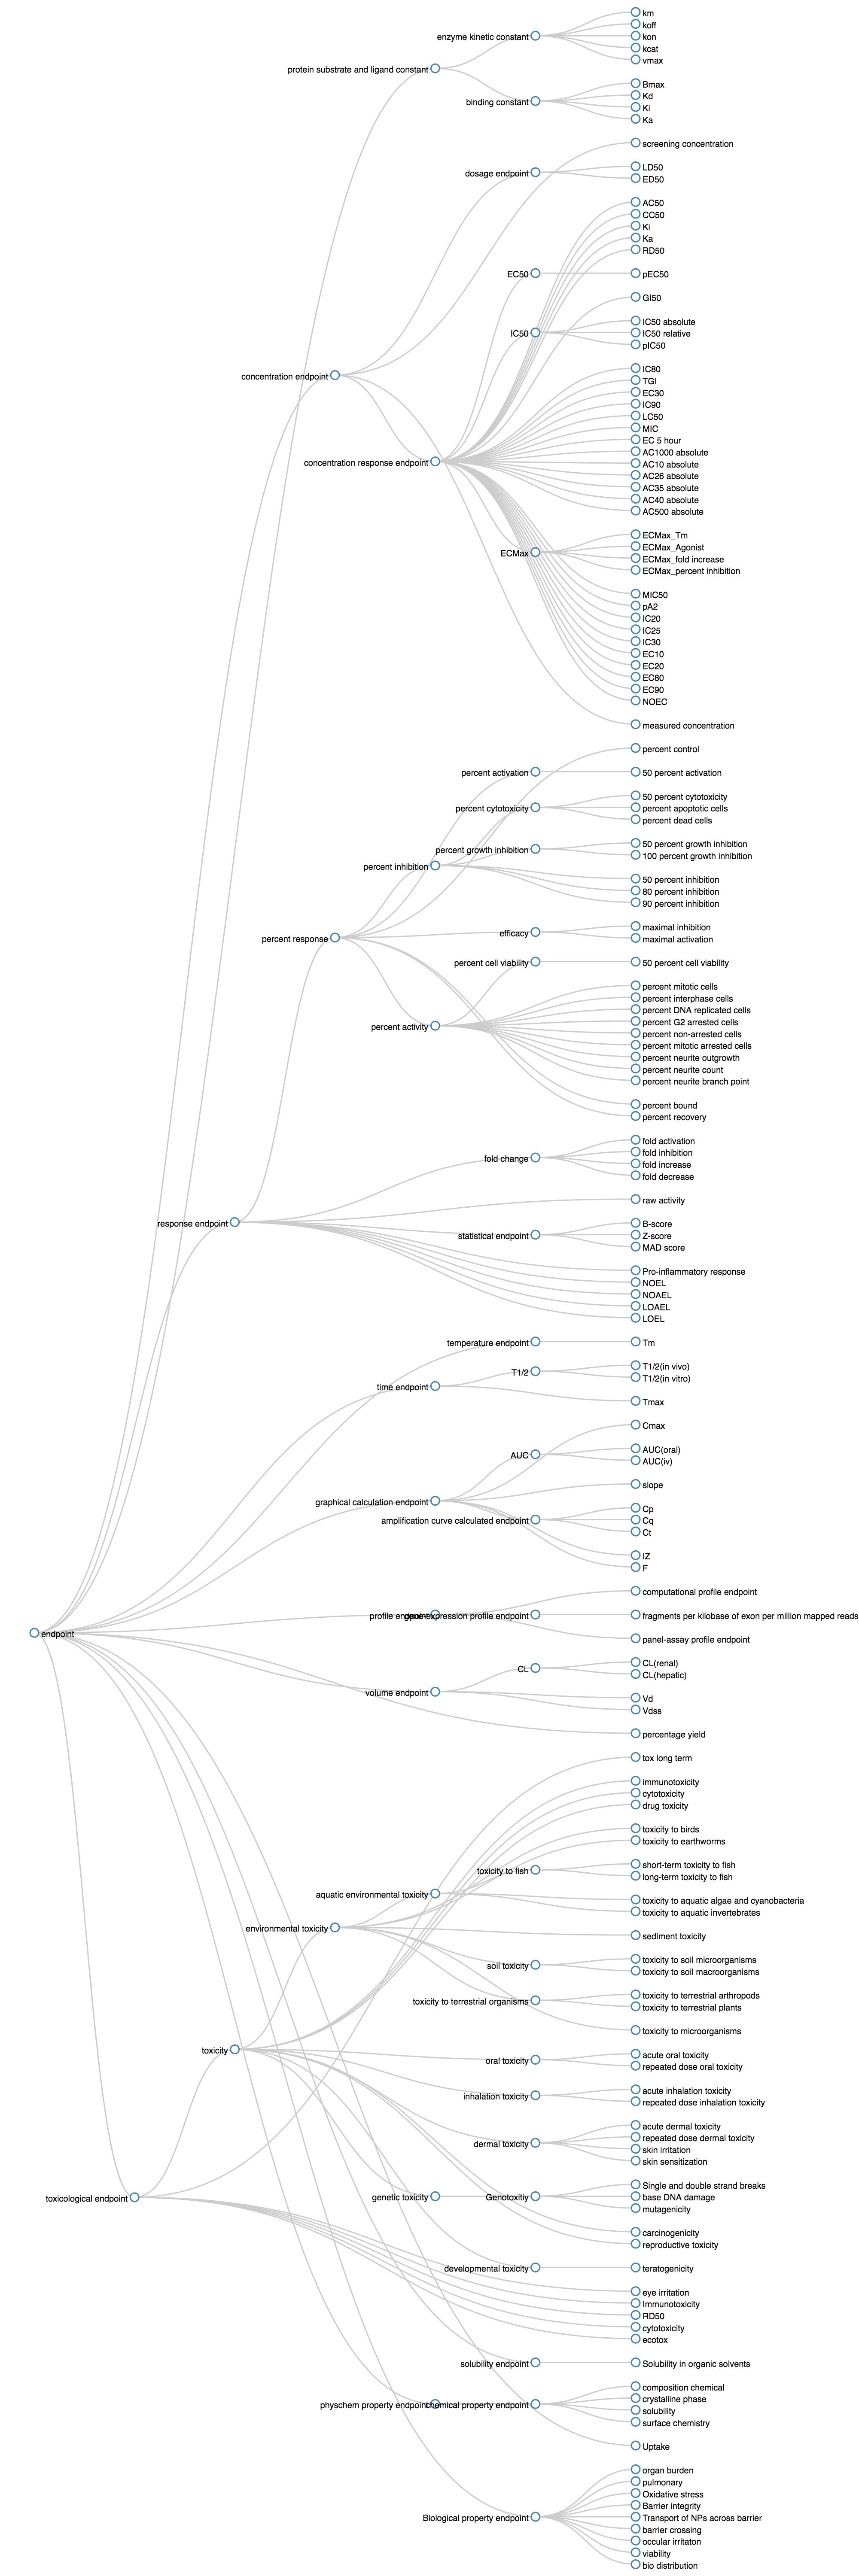
\includegraphics[scale=0.35,trim={20cm 0 0 0},clip]{onto-viewer-dendogram-1.png}
    \end{textblock}
    \begin{textblock}{40}(3,96)
      \small Figure 1: Dendogram
    \end{textblock}
    
    \begin{textblock}{62}(20,18)
      \justifying
      \begin{block}{Use case 1: Investigate the eNanoMapper Ontology}
        Assuming that we are interested in \emph{toxicological endpoints} we execute the template SPARQL query to receive results either as a static graphic named \emph{Dendogram} (Figure 1) or as a interactive graphic named \emph{Sunburst} (Figure 2). To get all depending information to our subject we can now use the SPARQL interface (Figure 4) and write another query. We are always able to refine our query from step 2 or investigate direct any kind of URIs from the result (Figure 5).
        \begin{figure}
          \hspace{-0.15\textwidth}
          \begin{subfigure}[c]{0.3\textwidth}
            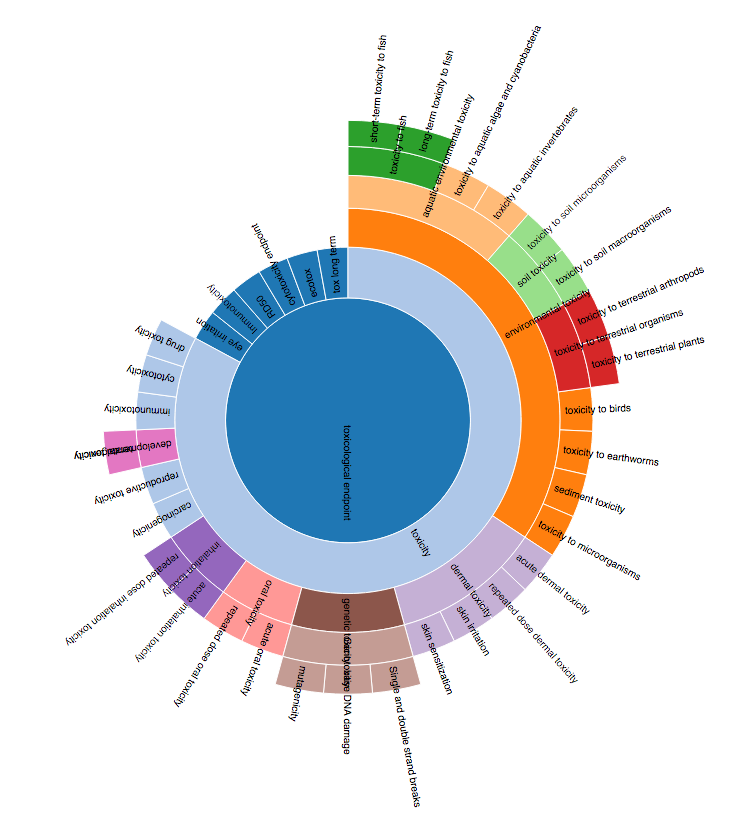
\includegraphics[width=\textwidth,keepaspectratio]{onto-use-case-1a.png}
            \caption{Figure 2: Sunburst. Result for \emph{toxicological endpoint} search.}
          \end{subfigure}
          \hspace{0.25\textwidth}
          \begin{subfigure}[c]{0.2\textwidth}
            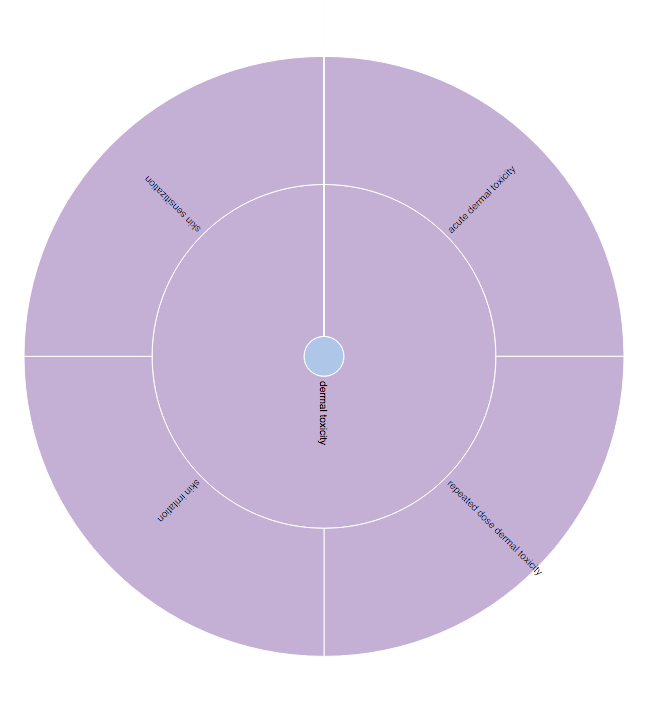
\includegraphics[width=\textwidth,keepaspectratio]{onto-use-case-1b.png}
            \caption{Figure 3: Sunburst. Interactive zoom on 'dermal toxicity' endpoint.}
          \end{subfigure}
        \end{figure}
        \vspace{0.05\textwidth}
        \begin{figure}
          %\centering
          \hspace{-0.1\textwidth}
          \begin{subfigure}[c]{0.3\textwidth}
            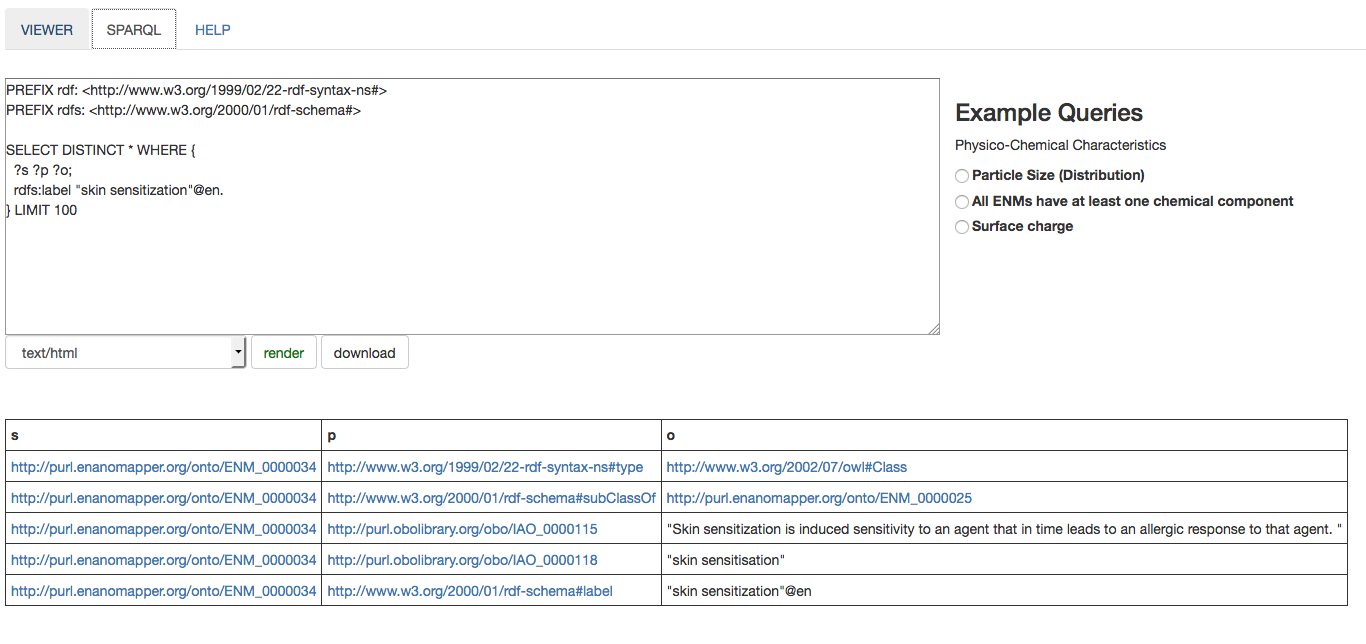
\includegraphics[width=\textwidth,keepaspectratio]{onto-use-case-1c.png}
            \caption{Figure 4: SPARQL interface. Take \emph{skin sensitization} subclass endpoint from Figure 3 for a detail query.}
          \end{subfigure}
          \hspace{0.2\textwidth}
          \begin{subfigure}[c]{0.3\textwidth}
            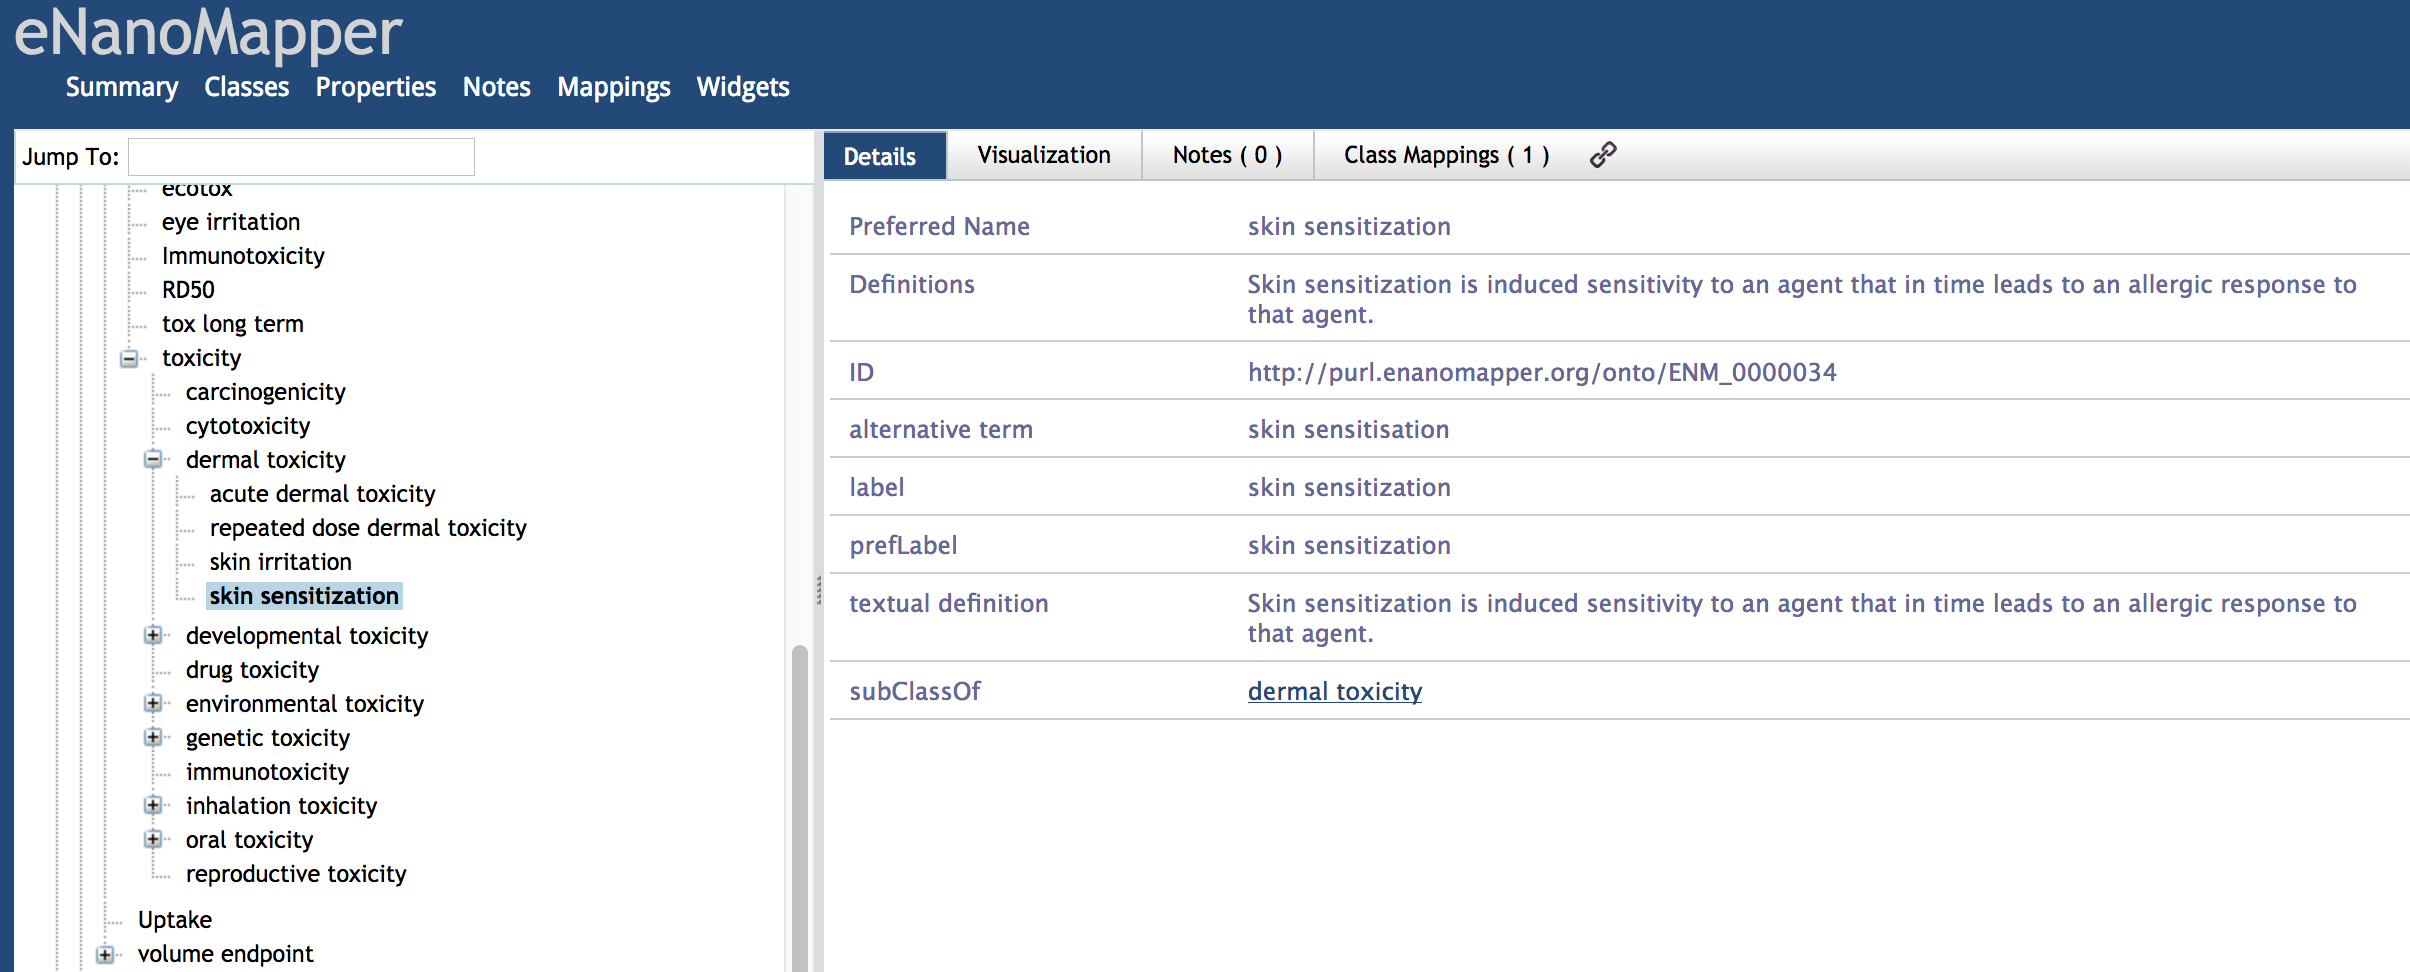
\includegraphics[width=\textwidth,keepaspectratio]{onto-use-case-1d.png}
            \caption{Figure 5: Following a link from query result in \emph{Figure 4} we get pointed to the eNanoMapper ontology on BioPortal.}
          \end{subfigure}
        \end{figure}
      \end{block}
    \end{textblock}

        
    \begin{textblock}{62}(20,70)
      \justifying
      \begin{block}{Use case 2: Investigate the eNanoMapper Data}
        Assuming that we want to investigate eNanoMapper nano material data we can simply choose one of the given SPARQL examples (Figure 1) as a starting point. In this case we are interessted in \emph{surface charge} and search for the zeta potential and its values. We receive a table with values and resource identifiers which point us direct to the resource page within eNanoMapper data service (Figure 7).
        \begin{figure}
          %\centering
          \vspace{0.05\textwidth}
          \hspace{-0.1\textwidth}
          \begin{subfigure}[c]{0.3\textwidth}
            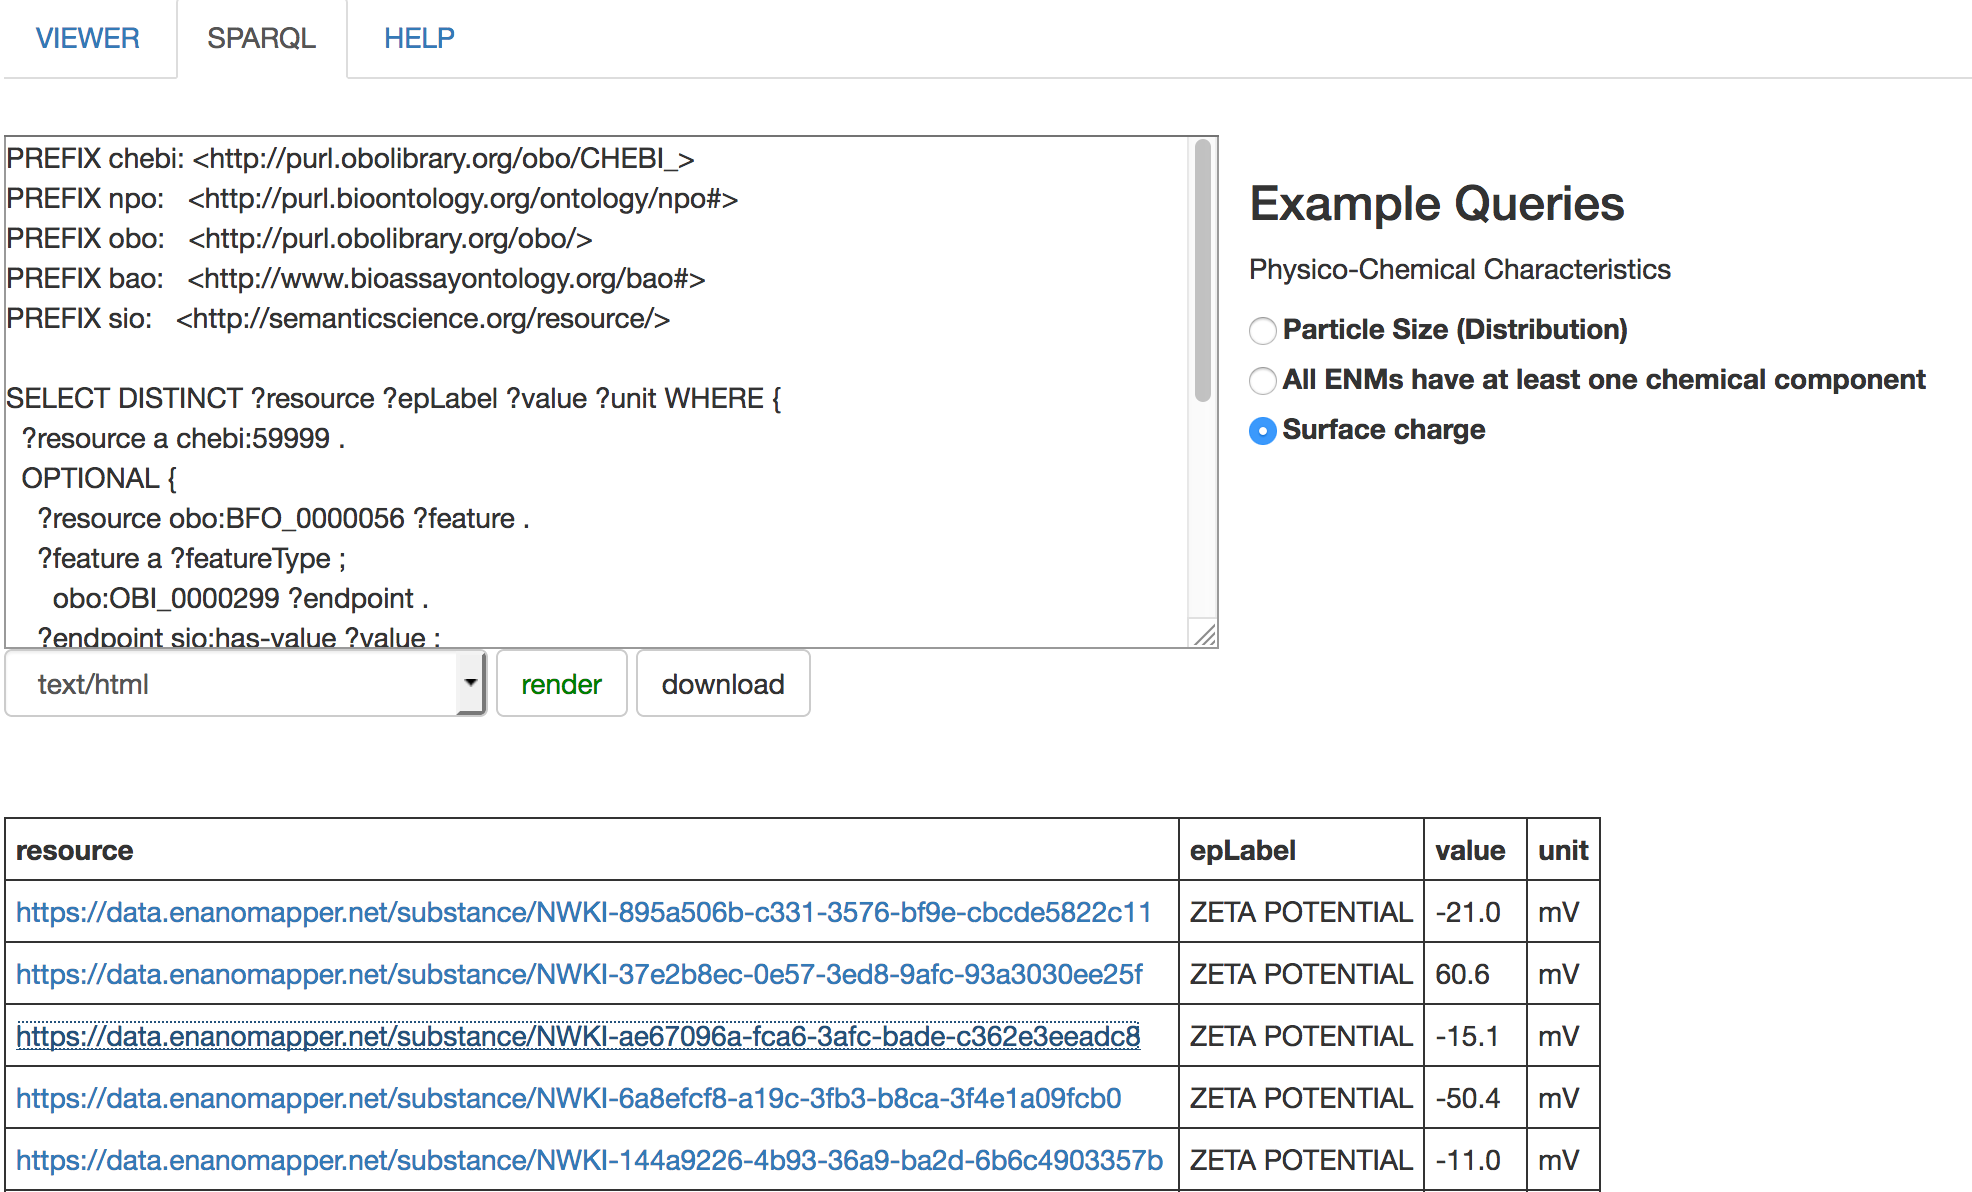
\includegraphics[width=\textwidth,keepaspectratio]{onto-use-case-2a.png}
            \caption{Figure 6: SPARQL interface. Choosen one of the "Physio-Chemical Characteristics" examples.}
          \end{subfigure}
          \hspace{0.2\textwidth}
          \begin{subfigure}[c]{0.4\textwidth}
            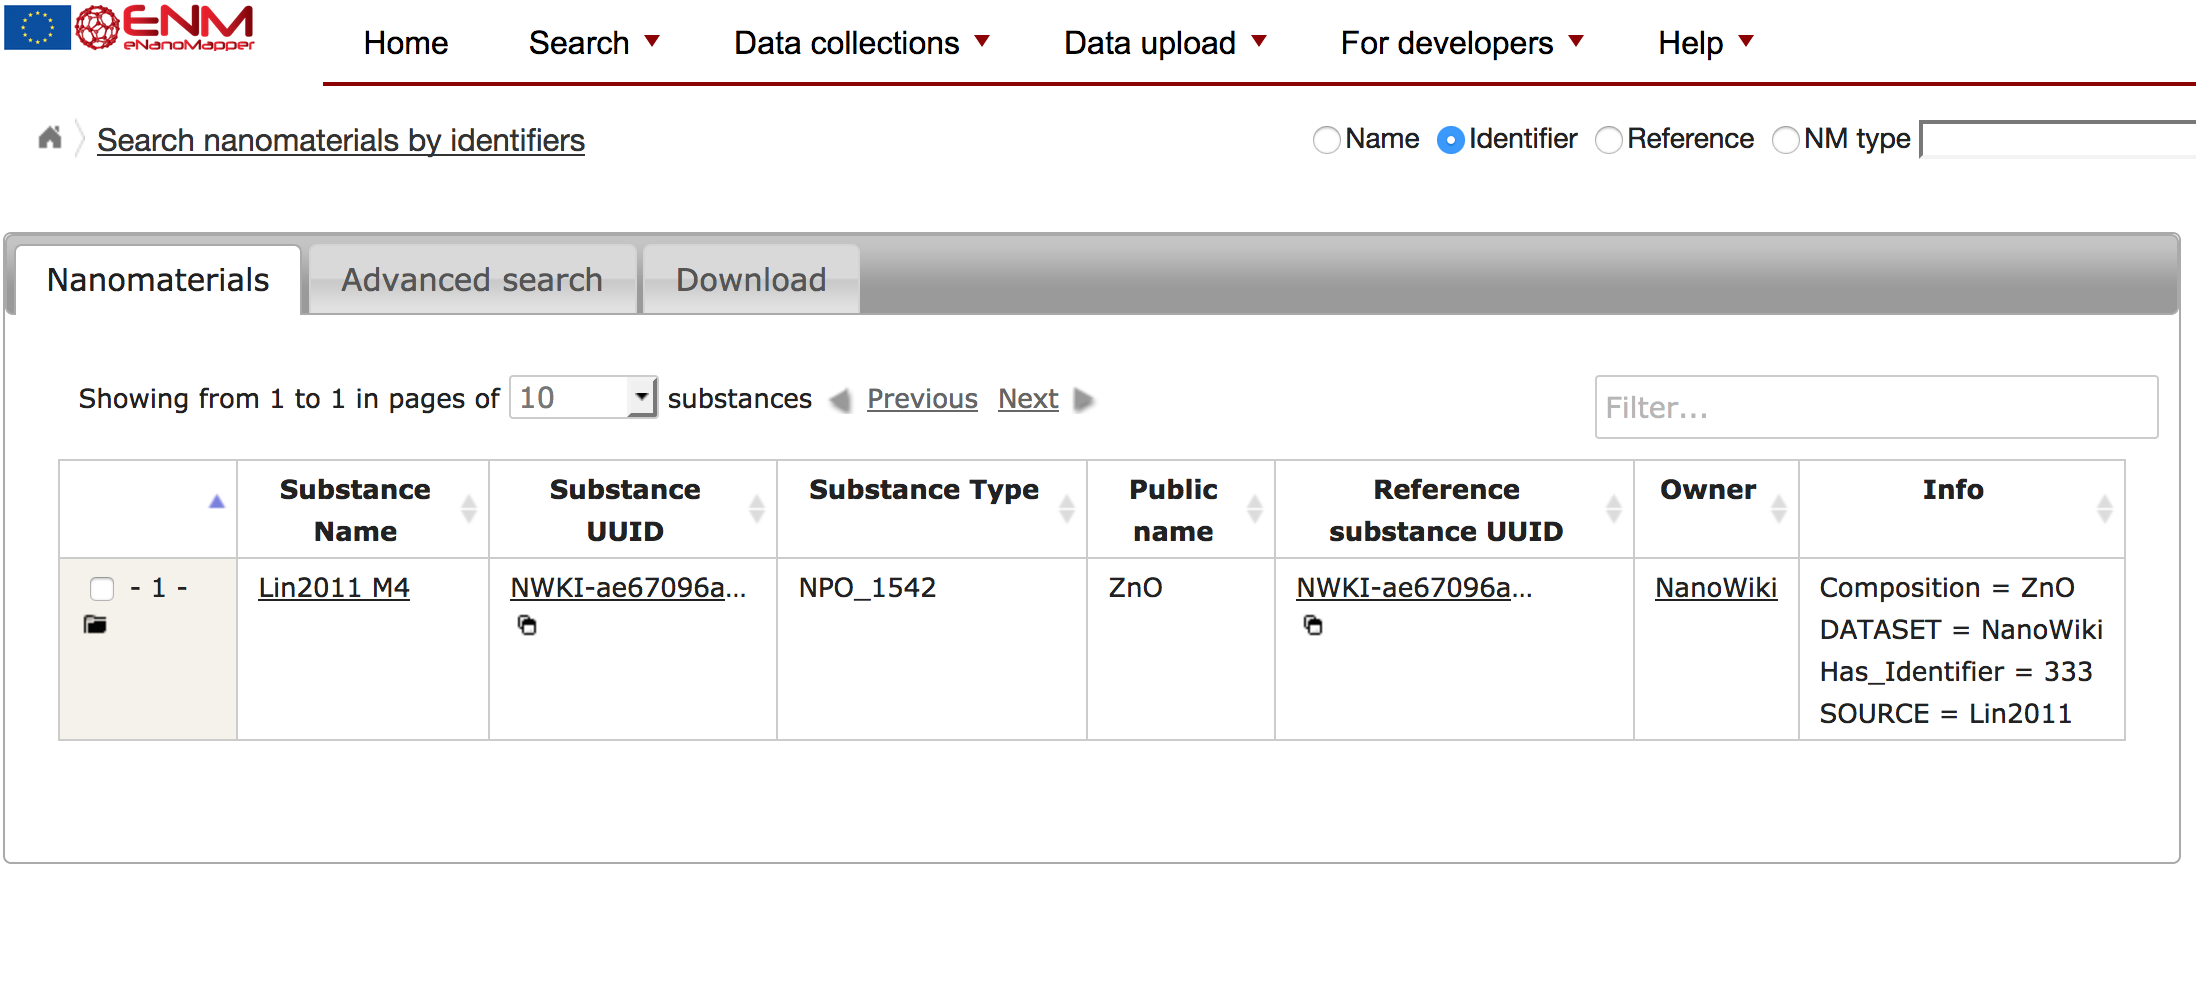
\includegraphics[width=\textwidth,keepaspectratio]{onto-use-case-2b.png}
            \caption{Figure 7: Follow link from query result in Figure 6 points to eNanoMapper data store.}
          \end{subfigure}
        \end{figure}
      \end{block}
    \end{textblock}
    
    \begin{textblock}{40}(1,100)
      \begin{exampleblock}{Links}
        \input{./markdown_blocks/ontoviewer_links}
      \end{exampleblock}
    \end{textblock}

    \begin{textblock}{40}(42.5,100)
      \begin{block}{References}
        \small\bibliography{references}
      \end{block}
    \end{textblock}

  \end{frame}

\end{document}
